%!tex root=./thesis.tex
\chapter{Faraday Complexity}
\label{cha:faraday}

\section{Faraday Complexity}
\label{sec:faraday-complexity}

This chapter is based on my to-be-submitted paper \emph{Interpretable Faraday Complexity Classification}, by M. J. Alger, C. S. Ong, J. D. Livingston, J. L. Nabaglo, N. M. McClure-Griffiths, and O. I. Wong.

I haven't finished this paper yet but I want to know what it looks like in the thesis!

\section{Introduction}
\label{sec:intro}

  As polarised light from distant galaxies makes its way to us, magnetised plasma along the way can cause the polarisation angle to rotate due to the Faraday effect. The amount of rotation is called the Faraday depth, and is related to the electron density and the magnetic field strength:
  \begin{equation}
      \phi = 0.81 \int_{\mathrm{there}}^{\mathrm{here}} n_e(\vec r) \vec B(\vec r) \cdot \mathrm{d}\vec{r}\ \mathrm{rad}\ \mathrm{m}^{-2}.
  \end{equation}
  Here $\phi$ is the Faraday depth, $n_e$ is the electron density in $\mathrm{cm}^{-3}$, $\vec B$ is the magnetic field in $\upmu$G, and $\mathrm{d}\vec r$ is the infinitesimal path length in pc \citep{brentjens_faraday_2005}. Multiple Faraday depths may exist along one line-of-sight, and if a polarised source is observed at multiple wavelengths then these multiple depths can be disentangled. This can provide insight into the polarised structure of the source.

  Faraday rotation measure synthesis (RM synthesis) is a technique for characterising the polarised intensity of an observation as a distribution of Faraday depths $\phi$, called a `Faraday dispersion function' (FDF) or a `Faraday spectrum'. It was introduced by \citet{brentjens_faraday_2005} as a way to rapidly and reliably analyse the polarisation structure of complex and high-Faraday depth polarised observations. The relationship between the observed complex polarised surface brightness $P(\lambda^2)$ and the underlying FDF $F(\phi)$ is similar to a Fourier transform:

  \begin{equation}
      \label{eq:f-to-p}
      P(\lambda^2) = \int_{-\infty}^{\infty} F(\phi) e^{2i\phi\lambda^2}\ \mathrm{d}\phi.
  \end{equation}

  A `Faraday simple' observation is one for which the peak Faraday depth of the FDF is simply the slope of the polarisation angle $\chi(\lambda^2)$ (called the `rotation measure' or RM). All Faraday simple observations can be modelled as a polarised source with a magnetised thermal plasma \citep[a `Faraday screen';][]{brentjens_faraday_2005,anderson_broadband_2015} between the observer and the source. A `Faraday complex' observation is one which is not Faraday simple, and may differ from a Faraday simple source due to plasma emission or composition of multiple screens \citep{brentjens_faraday_2005}. Identifying when an observation is Faraday complex is an important problem in polarised surveys. We introduce a simple, interpretable method for estimating Faraday complexity and demonstrate its effectiveness on both simulated and real data. Using simulated data, we compare our method to the state-of-the-art Faraday moments and CNN Faraday complexity estimation methods.

\section{Faraday dispersion functions}

  \begin{figure}
    % 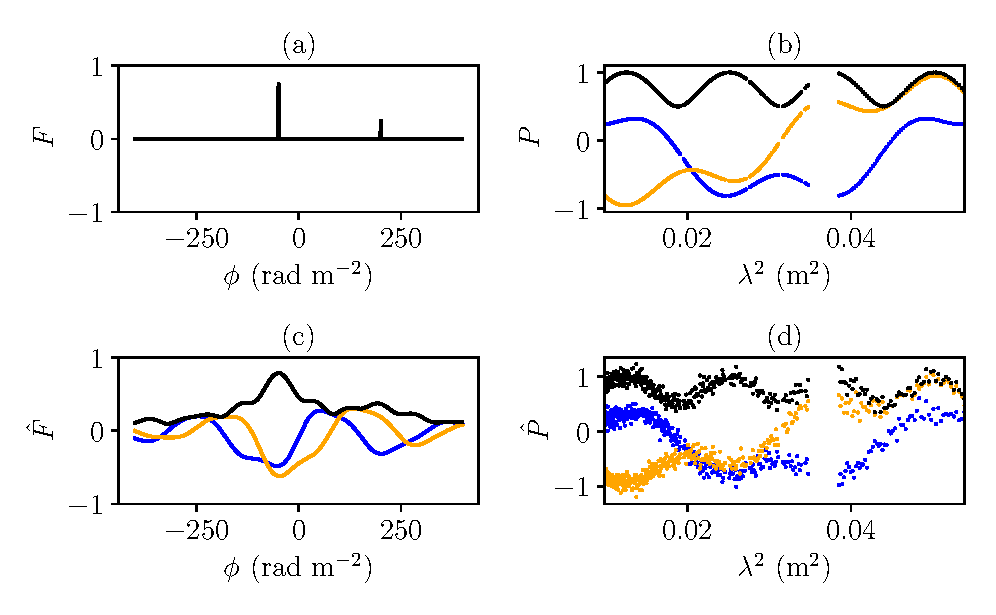
\includegraphics[width=\linewidth]{images/spectra.pdf}
    \caption{A FDF and its corresponding polarised spectra: (a) groundtruth FDF $F$, (b) groundtruth polarised spectrum $P$, (c) noisy observed FDF $\hat F$, (d) noisy polarised spectrum $\hat P$. Blue and orange mark real and imaginary components respectively.}
  \end{figure}

  For the purposes of this paper, a FDF is a function $F : \mathbb R \to \mathbb C$ from Faraday depth $\phi$ to complex polarisation. The FDF is implicitly defined and related to the polarised spectrum $P : \mathbb R \to \mathbb C$ by \autoref{eq:f-to-p}. We assume that $F$ has no noise and no observational limitations, and so $P$ also has no noise or limitations. We instead define $\hat F$ and $\hat P$ as the noisy, observed FDF and polarisation respectively. $\hat P$ is observed directly, and $\hat F$ is defined in terms of $\hat P$ by RM synthesis:
  \begin{equation}
      \label{eq:rm-synthesis}
      \hat F(\phi) = K^{-1} \int_{0}^{\infty} W(\lambda^2) \hat P(\lambda^2) e^{-2i\phi\lambda^2}\ \mathrm{d}\lambda^2.
  \end{equation}
  $W(\lambda^2)$ is a weighting function, which we assume to be 1 if polarisation was observed at $\lambda^2$ and 0 for all other values. This is called `uniform weighting' and is the most common weighting function for RM synthesis, but other weighting functions are possible in analogy with radio synthesis imaging. $K$ is a normalisation constant:
  \begin{equation}
    \label{eq:k}
    K = \int_{0}^\infty W(\lambda^2)\ \mathrm{d}\lambda^2.
  \end{equation}
  \citet{brentjens_faraday_2005} show that when there is no noise, the observed FDF $\hat F$ is related to the groundtruth $F$ by convolution with a function $R$ called the `rotation measure spread function' or RMSF:
  \begin{equation}
    \label{eq:hat-f-r-ast-f}
    \hat F(\phi) \overset{\text{no noise}}{=} (R \ast F)(\phi)
  \end{equation}
  $R$ is defined as the normalised Fourier transform of $W$:
  \begin{equation}
    \label{eq:rmsf}
    R(\phi) = K^{-1} \int_{0}^{\infty} W(\lambda^2) e^{-2i\phi\lambda^2}\ \mathrm{d}{\lambda^2}.
  \end{equation}
  If the noise in $\hat P$ is wavelength-independent Gaussian, then $\hat F$ can be represented as a Gaussian process with kernel $R$ and mean $R \ast F$. In other words,
  \begin{equation}
    \label{eq:hat-f-distribution}
    p(\hat F) = \mathcal N_c(\hat F \mid R \ast F, \Sigma(\phi, \varphi))
  \end{equation}
  where the covariance $\Sigma$ is
  \begin{equation}
    \Sigma(\phi, \varphi) = \int_{-\infty}^\infty R(\vartheta - \phi) R(\vartheta - \varphi)\ \mathrm{d}\vartheta.
  \end{equation}
  Note that there are two sources of noise in the observed FDF. The first arises from noise in $\hat P$. The second arises from the incomplete sampling of $\hat P$ as represented by $W$. In summary, $F$ is the groundtruth FDF, $P$ is the groundtruth polarisation spectrum, $\hat P$ is the noisy/observed polarisation spectrum, $\hat F$ is the noisy/observed FDF, $W$ is a weighting function and $R$ is the RMSF. Observations $\hat F$ can be simulated by either performing RM synthesis on simulated polarisation spectra or by drawing from \autoref{eq:hat-f-distribution}.

  % Assuming uncorrelated Gaussian noise in the polarised signal, $\hat P$ is drawn from a degenerate Gaussian process:
  % \begin{equation}
  %   \label{eq:hat-p}
  %   \hat P(\lambda^2) \sim W(\lambda^2) \left[P(\lambda^2) + \epsilon(\lambda^2)\right].
  % \end{equation}
  % $\epsilon : \mathbb R \to \mathbb C$ is a zero-mean, ergodic, and uncorrelated (white) Gaussian process, and $W(\lambda^2)$ is 1 if we observed at $\lambda^2$ and 0 for all other values. Note that we assume uniform weighting for RM synthesis throughout this paper. Also, in general, the Gaussian noise in $\hat P$ may not be uncorrelated and may not be ergodic.

  \subsection{Assumptions on polarised sources}

    We assume that all polarised sources are composed of either one or two Faraday screens. This accounts for almost all actual sources \citep{anderson_broadband_2015} and extension to three screens would cover most of the remainder \citep{osullivan_broad-band_2017}. This means that every groundtruth FDF is of the form
    \begin{equation}
        \label{eq:true-fdf}
        F(\phi) = A_0 \delta(\phi - \phi_0) + A_1 \delta(\phi - \phi_1).
    \end{equation}
    With this model, a Faraday simple source is one which has $A_0 = 0$, $A_1 = 1$, or $\phi_0 = \phi_1$. Applying \autoref{eq:f-to-p}, every groundtruth polarised spectrum is of the form
    \begin{equation}
        \label{eq:true-pol}
        P(\lambda^2) = A_0 e^{2i\phi_0\lambda^2} + A_1 e^{2i\phi_1\lambda^2}.
    \end{equation}
    We assume that polarised observations $\hat P$ have complex Gaussian noise $\epsilon(\lambda^2)$:
    \begin{align}
        \label{eq:pol-noise}
        \epsilon(\lambda^2) \sim \mathcal N_c(0, \sigma(\lambda^2)^2),
    \end{align}
    and that $\sigma(\lambda^2)^2$ is constant.

  \subsection{Simulating observed FDFs}
  \label{sec:simulated-fdfs}

    To simulate observed FDFs we follow the method of \citet{brown_classifying_2018}. $F$ is approximated on the domain $[\phi_{\min}, \phi_{\max}]$ by a vector $\vec F \in \mathbb R^d$:
    \begin{equation}
      \label{eq:vec-f}
      \vec F_j = \sum_{k = 0}^1 A_k \delta(\phi_{\min} + j \delta \phi - \phi_k)
    \end{equation}
    where $\delta\phi = (\phi_{\max} - \phi_{\min}) / d$.
    $\vec F$ is sampled by uniformly sampling its parameters:
    \begin{align}
      \label{eq:model-distributions}
      % p(\phi_0, \phi_1, A_0, A_1) = \frac{1}{(\phi_{\max} - \phi_{\min})^2} \begin{cases}
      %   1 & \phi_{0,1} \in [\phi_{\min} \phi_{\max}],\\
      %     & A_{0, 1} \in [0, 1];\\
      %   0 & \mathrm{otherwise}.
      % \end{cases}
      % p(\phi_k) &= \frac{1}{\phi_{\max} - \phi_{\min}} \begin{cases}
      %   1 & \phi_k \in [\phi_{\min} \phi_{\max}],\\
      %   0 & \mathrm{otherwise};
      % \end{cases}\\
      % p(A_k) &= \begin{cases}
      %   1 & \phi_k \in [0, 1],\\
      %   0 & \mathrm{otherwise};
      % \end{cases}
      \phi_k &\in [\phi_{\min}, \phi_{\min} + \delta\phi, \dots, \phi_{\max}]\\
      A_k &\sim \mathcal U(0, 1).
    \end{align}
    We assume that the total polarisation is 1: real observations can be scaled to this by dividing by their total polarisation. We then generate a vector polarisation spectrum $\vec P \in \mathbb R^m$ from $\vec F$ using a discretised \autoref{eq:f-to-p}:
    \begin{equation}
      \label{eq:discrete-f-to-p}
      \vec P_\ell = \sum_{j = 0}^{j} F_j e^{2i(\phi_{\min} + j\delta_\phi)\lambda^2_\ell}\ \mathrm{d}\phi.
    \end{equation}
    $\lambda^2_\ell$ is the discretised value of $\lambda^2$ at the $\ell$th index of $\vec P$. These values can be treated as the channel wavelengths at which the polarisation spectrum was observed. We then add Gaussian noise with variance $\sigma^2$ to each element of $\vec P$ to obtain a discretised noisy observation $\hat{\vec{P}}$. Finally, we perform RM synthesis using the Canadian Initiative for Radio Astronomy Data Analysis \texttt{RM} package\footnote{\url{https://github.com/CIRADA-Tools/RM}}, which is a \texttt{Python} module that implements a discrete version of RM synthesis:
    \begin{equation}
      \label{eq:discrete-rm-synthesis}
      \hat{\vec{F}}_j = m^{-1} \sum_{\ell = 1}^m \vec{\hat P}_\ell e^{-2i(\phi_{\min} + j\delta_\phi)\lambda^2_\ell}.
    \end{equation}

\section{Faraday complexity}

    Faraday complexity is an obsevational property of a source: if multiple Faraday depths are observed within the same apparent source (e.g. due to multiple lines-of-sight being combined within a beam), then the source is complex, and otherwise it is simple. There are multiple ways to estimate Faraday complexity, including detecting non-linearity in $\chi(\lambda^2)$ \citep{goldstein84faraday}, change in fractional polarisation as a function of frequency \citep{farnes14broadband}, non-sinusoidal variation in fractional polarisation in Stokes $Q$ and $U$ \citep{osullivan12agn}, counting components in the FDF \citep{law11faraday}, the method of Faraday moments \citep{anderson_broadband_2015,Brown11report}, and deep convolutional neural network classifiers \citep[CNNs;][]{brown_classifying_2018}. The first four methods have significant drawbacks \citep[see][]{anderson_broadband_2015}. Faraday moments and CNNs are the state-of-the-art methods which we will compare to in this paper.

    \subsection{Methods for estimating complexity}
    \label{sec:existing-methods}

        Faraday moments \citep{Brown11report,anderson_broadband_2015} and CNNs \citep{brown_classifying_2018} are the two methods for estimating Faraday moments that we will consider here.

        \subsubsection{Faraday moments}
        \label{sec:faraday-moments}
            The method of Faraday moments requires the FDF to be deconvolved using \texttt{RM-CLEAN} \citeneeded{}, a deconvolution program in analogy to \texttt{CLEAN} used in radio synthesis imagery. The estimated deconvolved FDF is a sum of delta functions called `clean components'. The second moment is computed over these components and thresholded to determine if a source is Faraday complex. The second moment $\varsigma_{\mathrm{mom}}$ is defined as
            \begin{equation}
                \varsigma_{\mathrm{mom}}^2 = K_C^{-1} \sum_{i = 1}^N (\phi_i - \langle \phi \rangle)^2 |C_i|
            \end{equation}
            where $N$ is the number of clean components, $C_i$ is the complex intensity of the $i$th clean component, $K_C$ is the normalisation:
            \begin{equation}
                K_C = \sum_{i = 1}^N |C_i|,
            \end{equation}
            and $\langle \phi \rangle$ is the mean depth of the clean components:
            \begin{equation}
                \langle \phi \rangle = K_C^{-1} \sum_{i = 1}^N \phi_i |C_i|.
            \end{equation}
            Drawbacks of this method include the need to determine a threshold and the care required to produce the clean components. In particular, deconvolution is a challenging process and works poorly on noisy data. Significant oversight is required to clean large quantities of sources, which limits its usage in large surveys.

            For our model spectra (\autoref{eq:true-fdf}) we can treat each delta function as a clean component and hence write down the Faraday moment for a FDF in the ideal, fully-observed scenario (i.e. no noise and an infinitely thin RMSF):
            \begin{equation}
                \label{eq:model-moment}
                \varsigma_{\mathrm{mom}}^2 = \frac{A_0A_1}{(A_0 + A_1)^2} (\phi_0 - \phi_1)^2.
            \end{equation}
            This has units of rad~m$^{-2}$.

        \subsubsection{Convolutional neural networks}
        \label{sec:cnns}

            todo

            defines $\varsigma_{\mathrm{cnn}}$.

    \subsection{Faraday complexity scores}
    \label{sec:scores-method}
    
        In existing literature the `Faraday complexity' of a source is a binary property: either a source is Faraday simple, and composed of a single Faraday screen; or it is Faraday complex, and composed of multiple Faraday screens\footnote{A complex source may instead be Faraday thick, but in our model we assume that this is well-approximated by two screens.}. We propose to measure Faraday complexity as a real-valued quantity, where a complexity of zero indicates that a source is simple and the quantity increases as the source becomes less simple. We call such a quantity a `Faraday complexity score'. There are many ways such a score could be defined, but if it is to be a meaningful measure of Faraday complexity, then a score must have certain properties.

        A Faraday complexity score should be:
        \begin{itemize}
            \item phase-invariant,
            \item translationally invariant in Faraday depth,
            \item zero for Faraday simple sources (i.e. when $A_0 = 0$, $A_1 = 0$, or $\phi_0 = \phi_1$),
            \item symmetric in components (i.e. swapping $A_0 \leftrightarrow A_1$ and $\phi_0 \leftrightarrow \phi_1$ should not change the complexity score),
            \item scale-invariant, i.e. scaling $A_0$ and $A_1$ by the same amount should not change the complexity score,
            \item increasing as $A_0$ and $A_1$ become closer to each other, and
            \item increasing as screen separation $|\phi_0 - \phi_1|$ increases.
        \end{itemize}

        The second moment $\varsigma_{\mathrm{mom}}$ fulfils these properties, and so is a valid complexity score. However, it can only be calculated on the true FDF, or the clean component estimation of the true FDF. It would be useful to have a complexity measure which can be computed on the noisy, observed FDF.

        We propose to measure Faraday complexity as the divergence of an observed FDF from the manifold of simple FDFs. Parametrise the manifold by $\phi_s$, using the scale invariance of Faraday complexity scores to set the intensity to 1, for both observed and model FDFs:
        \begin{align}
            F_{\mathrm{simple}}(\phi; \phi_s) &= \delta(\phi - \phi_s)\\
            \hat F_{\mathrm{simple}}(\phi; \phi_s) &= R(\phi - \phi_s).
        \end{align}
        The complexity of a model FDF $F$ would then be
        \begin{equation}
            \label{eq:complexity-model}
            \varsigma_D(F) = \min_{\phi_s \in \mathbb{R}} D\infdivx{F(\phi)}{F_{\mathrm{simple}}(\phi; \phi_s)}
        \end{equation}
        and similarly the complexity of an observed FDF $\hat F$ would be
        \begin{equation}
            \label{eq:complexity-observed}
            \varsigma_D(\hat F) = \min_{\phi_s \in \mathbb{R}} D\infdivx{\hat F(\phi)}{\hat F_{\mathrm{simple}}(\phi; \phi_s)}.
        \end{equation}
        $D$ is a divergence: a non-negative functional that is zero if and only if its arguments are the same. A divergence is like a distance, but without the need to fulfil a triangle inequality or symmetry. We have the freedom to choose different divergence functionals for model and observed spectra: these may not be the same as the convolution with the RMSF distorts the space of FDFs. The `correct' choice of divergence represents a way to measure distance on the space of FDFs and hence defines a meaningful geometry on this space.

        One choice of divergence is the 2-Wasserstein distance $D_{W_2}$ \citeneeded{}. This is usually defined on probability distributions, but can be extended to one-dimensional complex functions $A$ and $B$ by normalising them:
        \begin{align}
          \label{eq:w2}
          D_{W_2}\infdivx{A}{B}^2 &= \inf_{\gamma \in \Gamma(A, B)} \iint_{\phi_{\min}}^{\phi_{\max}} |x - y|^2\ \mathrm{d}\gamma(x, y) \\
          \label{eq:normalised}
          \tilde A(\phi) &= \frac{|A(\phi)|}{\int_{\phi_{\min}}^{\phi_{\max}} |A(\theta)|\ \mathrm{d}\theta}\\
          \tilde B(\phi) &= \frac{|B(\phi)|}{\int_{\phi_{\min}}^{\phi_{\max}} |B(\theta)|\ \mathrm{d}\theta}
        \end{align}
        where $\Gamma(A, B)$ is the set of couplings of $A$ and $B$, i.e. the set of joint probability distributions that marginalise to $A$ and $B$. This can be interpreted as the minimum cost to `move' one probability distribution to the other, where the cost of moving one unit of probability mass is the squared distance it is moved. Choosing the 2-Wasserstein distance to measure complexity of a model FDF yields the Faraday moment from \autoref{eq:model-moment}:
        \begin{align}
            \varsigma_{W_2}(F) &= \min_{\phi_s \in \mathbb{R}} D_{W_2}\infdivx{F(\phi)}{F_{\mathrm{simple}}(\phi; \phi_s)}\\
                &= \left(\frac{A_0A_1}{(A_0 + A_1)^2} (\phi_0 - \phi_1)^2\right)^{1/2}.
        \end{align}
        The minimising $\phi_s$ is the weighted mean of the FDF: precisely the Faraday depth that would be measured if the Faraday space resolution is too low to distinguish the two components. This provides an interpretation of Faraday moments as a distance from the simple manifold in the case where there is no RMSF.

        The 2-Wasserstein distance could also be used to measure complexity of observed FDFs, but other divergences may provide better results. We investigate four choices of divergence: Euclidean distance (\autoref{eq:euclidean-distance}), Kullback-Leibler (KL) divergence (\autoref{eq:kl-divergence}), Itakura-Saito (IS) divergence (\autoref{eq:is-divergence}), and 2-Wasserstein (W$_2$) distance (\autoref{eq:w2}). We compare their complexity scores on observed FDFs to the complexity scores on the equivalent model FDFs using the Faraday moment.
        \begin{align}
          \label{eq:euclidean-distance}
          D_{\mathrm{Euc}}\infdivx{A}{B} &= \left(\frac{\int_{\phi_{\min}}^{\phi_{\max}} (|A(\phi)| - |B(\phi)|)^2\ \mathrm{d}\phi}{\phi_{\max}-\phi_{\min}}\right)^{1/2}\\
          \label{eq:kl-divergence}
          D_{\mathrm{KL}}\infdivx{A}{B} &= \int_{\phi_{\min}}^{\phi_{\max}} \tilde A(\phi) \log \frac{\tilde A(\phi)}{\tilde B(\phi)}\ \mathrm{d}\phi\\
          \label{eq:is-divergence}
          D_{\mathrm{IS}}\infdivx{A}{B} &= \frac{\int_{\phi_{\min}}^{\phi_{\max}} \frac{\tilde A(\phi)}{\tilde B(\phi)} - \log \frac{\tilde A(\phi)}{\tilde B(\phi)} - 1\ \mathrm{d}\phi}{\phi_{\max}-\phi_{\min}}
        \end{align}

        For vector discretisations of FDFs as defined in \autoref{sec:simulated-fdfs}, we define the following approximations:
        \begin{align}
          \label{eq:euclidean-distance-discrete}
          D_{\mathrm{Euc}}\infdivx{\vec A}{\vec B} &= \left(\delta\phi \sum_{j = 1}^d (|\vec A_j| - |\vec B_j|)^2\right)^{1/2}\\
          \label{eq:kl-divergence-discrete}
          D_{\mathrm{KL}}\infdivx{\vec A}{\vec B} &= \delta\phi \sum_{j = 1}^d \tilde{\vec A}_j \log \frac{\tilde{\vec A}_j}{\tilde{\vec B}_j}\\
          \label{eq:is-divergence-discrete}
          D_{\mathrm{IS}}\infdivx{\vec A}{\vec B} &= \delta\phi \sum_{j = 1}^d \left(\frac{\tilde{\vec A}_j}{\tilde{\vec B}_j} - \log \frac{\tilde{\vec A}_j}{\tilde{\vec B}_j} - 1\right)
        \end{align}
        where
        \begin{align}
          \tilde{\vec A}_j &= \frac{|\vec A_j|}{\sum_{k = 1}^d |\vec A_k|}\\
          \tilde{\vec B}_j &= \frac{|\vec B_j|}{\sum_{k = 1}^d |\vec B_k|}.
        \end{align}
        We calculate the 2-Wasserstein distance using \texttt{Python Optimal Transport}, which uses a method summarised in \autoref{sec:pot}.

\section{Experiment: No noise}

  \begin{figure*}
    \centering
    % \includegraphics[width=\linewidth]{images/complexities_abcd_3d.pdf}
    % \includegraphics[width=0.5\linewidth]{images/complexities_e_3d.pdf}
    \caption{Faraday complexity scores derived from different divergences. All plots are shown with arbitrary linear scales.}
    \label{fig:no-noise-complexities}
  \end{figure*}
  
  We begin by examining the behaviour of different Faraday complexity scores in the case where there is no noise, i.e. $\epsilon = 0$. In this setting the only difference between the groundtruth FDF and the observed FDF is the RMSF, so \autoref{eq:hat-f-r-ast-f} holds exactly. We generated 2~000 FDFs $\hat{\vec{F}}$ with different amplitudes and Faraday depths. For each divergence measure (Euclidean, KL, IS, and W$_2$) we calculated the corresponding Faraday complexity score for each FDF ($\varsigma_{\mathrm{Euc}}, \varsigma_{\mathrm{KL}}, \varsigma_{\mathrm{IS}},$ and $\varsigma_{\mathcal E}$ respectively) following \autoref{eq:complexity-observed}. We also calculated the Faraday moment ($\varsigma_{\mathrm{mom}}$, \autoref{eq:model-moment}) of the true FDFs $\vec F$. The Faraday complexity scores are plotted in \autoref{fig:no-noise-complexities}.

  Visually, W$_2$ best approximates the Faraday moment. This can be confirmed by computing the Spearman $\rho$ coefficient \citeneeded{} of the Faraday complexity score compared to the Faraday moment. W$_2$ has the highest Spearman $\rho$ of $\rho = 0.887$, followed by IS ($\rho = 0.862$), KL ($\rho = 0.753$), and Euclidean ($\rho = 0.466$).

\section{Experiment: Noise}

  Noise has an important relationship with Faraday complexity, so it is necessary to investigate the noisy case separately. We set $\sigma = 1$ i.e. our simulated polarised signals have a signal-to-noise ratio of 1, and simulate 10 noisy FDFs for each set of amplitudes and peak locations. This is unrealistically high, but we still have clear behaviour in Faraday complexity scores. As with the no-noise case, W$_2$ has the highest Spearman $\rho$ of $\rho = 0.900 \pm 0.001$, followed by IS ($\rho = 0.859 \pm 0.001$), KL ($\rho = 0.760 \pm 0.001$), and Euclidean ($\rho = 0.458 \pm 0.001$).


\begin{appendix}
  \section{2-Wasserstein begets Faraday moments}
  \label{sec:w2-to-faraday-moments}
    The 2-Wasserstein distance (\autoref{eq:w2}) gives the second Faraday moment (\autoref{eq:model-moment}) on a model FDF (\autoref{eq:true-fdf}). Let $\tilde F$ be the model FDF normalised as in \autoref{eq:normalised} and let $\tilde S$ be the normalised simple model FDF:
    \begin{align}
      \tilde F(\phi) &= \frac{A_0 \delta(\phi - \phi_0) + A_1 \delta(\phi - \phi_1)}{A_0 + A_1}\\
      \tilde S(\phi) &= \delta(\phi - \phi_s).
    \end{align}
    The set of couplings $\Gamma(\tilde F, \tilde S)$ is the set of all joint probability distributions $\gamma$ such that
    \begin{align}
      \int_{\phi_{\min}}^{\phi_{\max}} \gamma(\phi, \varphi)\ \mathrm{d}\phi &= \tilde S(\varphi),\\
      \int_{\phi_{\min}}^{\phi_{\max}} \gamma(\phi, \varphi)\ \mathrm{d}\varphi &= \tilde F(\phi).
    \end{align}
    The coupling that minimises the integral in \autoref{eq:w2} will be the optimal transport plan between $\tilde F$ and $\tilde S$. Since $\tilde F$ and $\tilde S$ are defined in terms of delta functions, the optimal transport problem reduces to a discrete optimal transport problem and the optimal transport plan is:
    \begin{equation}
      \gamma(\phi, \varphi) = \frac{A_0 \delta(\phi - \phi_0) + A_1 \delta(\phi - \phi_1)}{A_0 + A_1} \delta(\varphi - \phi_s).
    \end{equation}
    In other words, to move the probability mass of $\tilde S$ to $\tilde F$, a fraction $A_0/(A_0 + A_1)$ is moved from $\phi_s$ to $\phi_0$ and the complementary fraction $A_1/(A_0 + A_1)$ is moved from $\phi_s$ to $\phi_1$. Then:
    \begin{align}
      D_{W_2}\infdivx{\tilde F}{\tilde S}^2 &= \iint_{\phi_{\min}}^{\phi_{\max}} |\phi - \varphi|^2\ \mathrm{d}\gamma(\phi, \varphi)\\
        &= \frac{\iint_{\phi_{\min}}^{\phi_{\max}} (A_0 \delta(\phi - \phi_0) + A_1 \delta(\phi - \phi_1)) \delta(\varphi - \phi_s) (\phi - \varphi)^2\ \mathrm{d}\phi\ \mathrm{d}\varphi}{A_0 + A_1}\\
        &= \frac{\int_{\phi_{\min}}^{\phi_{\max}} (A_0 \delta(\phi - \phi_0) + A_1 \delta(\phi - \phi_1)) (\phi - \phi_s)^2\ \mathrm{d}\phi}{A_0 + A_1}\\
        &= \frac{A_0 (\phi_0 - \phi_s)^2 + A_1 (\phi_1 - \phi_s)^2}{A_0 + A_1}.
    \end{align}
    To obtain a Faraday complexity score (\autoref{eq:complexity-model}) we need to minimise this over $\phi_s$. Differentiate with respect to $\phi_s$ and set equal to zero to find
    \begin{equation}
      \phi_s = \frac{A_0 \phi_0 + A_1 \phi_1}{A_0 + A_1}.
    \end{equation}
    Substituting this back in, we find
    \begin{align}
      \varsigma_{W_2}(F)^2 &= \frac{A_0 (\phi_0 - \frac{A_0 \phi_0 + A_1 \phi_1}{A_0 + A_1})^2 + A_1 (\phi_1 - \frac{A_0 \phi_0 + A_1 \phi_1}{A_0 + A_1})^2}{A_0 + A_1}\\
        &= \frac{A_0 (A_1 (\phi_0 - \phi_1))^2 + A_1 (A_0 (\phi_1 - \phi_0))^2}{(A_0 + A_1)^3}\\
        &= \frac{A_0 A_1^2 (\phi_0 - \phi_1)^2 + A_0^2 A_1 (\phi_0 - \phi_1)^2}{(A_0 + A_1)^3}\\
        &= \frac{(A_0 A_1^2 + A_0^2 A_1) (\phi_0 - \phi_1)^2}{(A_0 + A_1)^3}\\
        &= \frac{A_0 A_1}{A_0 + A_1}(\phi_0 - \phi_1)^2
    \end{align}
    which is the Faraday moment.

  \section{Calculating W$_2$}
  \label{sec:pot}

\end{appendix}
